\documentclass[12pt,a4paper]{article}
\usepackage[utf8]{inputenc}
\usepackage{amsmath}
\usepackage{amsfonts}
\usepackage{amssymb}
\usepackage{float}
\usepackage{csvsimple}
\usepackage{enumerate}
\usepackage{hyperref}
\usepackage{graphicx}
\usepackage{gensymb}
\usepackage{txfonts}
\usepackage{listings}
\usepackage{cleveref}
\usepackage{xcolor}
\parindent 0px
\usepackage[none]{hyphenat}
\usepackage{listings} %Package for the enviroment in which we write code 
\usepackage[left=2cm,right=2cm,top=2cm]{geometry}
\pagenumbering{arabic}
%Some custom colours
\definecolor{codegreen}{rgb}{0,0.6,0}
\definecolor{codegray}{rgb}{0.5,0.5,0.5}
\definecolor{codepurple}{rgb}{0.58,0,0.82}
\definecolor{backgroundcolour}{rgb}{0.95,0.95,0.92}

%Shortcut for strings "Code" and "List of Code"
\renewcommand{\lstlistingname}{Code}
\renewcommand{\lstlistlistingname}{List of Code}

%This is the template for code styling, named as "mystyle"
\lstdefinestyle{mystyle}{
	backgroundcolor=\color{backgroundcolour},
	basicstyle=\ttfamily\small,
	commentstyle=\color{green!60!black},
	keywordstyle=\color{magenta},
	stringstyle=\color{blue!50!red},
	showstringspaces=false, 
	captionpos=b, %Position of caption top/bottom
	numbers=left,	%This command adds line numbers to the code
	%numberstyle=\footnotesize\color{gray}, %This command sets the colour of the line numbers
	%numbersep=10pt, %This command determines the separation of the line numbers from the main margin
	%stepnumber=2,
	tabsize=2,
	frame=single, %setting to select the frame for code ... options available {L,single,shadowbox}
	%framerule=1pt, %selecting the width of the frame
	%rulecolor=\color{red}, %selecting the colour of the frame
	breaklines=true,
	inputpath=code	
}

%%%%%%%%%%%%%%%%%%%%%%%%%%%%%%%%%%%%%%%%%%%%%%%%%%%%%%%%%%%%%%%%%%%%%%%%%%%%%%%%%%%%%%%%%%%%%%%%%%%%%%%%%%%%%%%%%%%%%%%%%%%%%%%%%%%%%%%%%%%%%%%%%%%%%%%%%%%%%%%%%%%%%%%%%%%%%%%%%%%%%%%%%%%%%%%%%%%%%%%%%%%%%%%%%%%%%%%%%%%%%%
\title{CS3523 : OPERATING SYSTEMS 2 \\ Programming Assignment 5}
\author{ANUDEEP RAO PERALA \\ CS21BTECH11043 }
\date{}

\begin{document}
	\maketitle
	
	\newpage
	
	\subsection*{\underline{PART A - Demand Paging}}
	\subsection*{Implementation :}

	\subsubsection*{1) mydemandPage.c}
\begin{itemize}
	\item Firstly we create \textbf{mydemandPage.c} which is responsible to execute when we call the user program \textbf{mydemandPage}.
	\item In this function we declare a global array, based on the pagetables generated for mapping this array to physical memory we do furthur analysis.
	\item To print the pagetables we call the function \textbf{pgtPrint()}.
\end{itemize}
	\subsubsection*{2) Makefile}
									\begin{lstlisting}[language=C, style = mystyle]
	UPROGS=\
	_cat\
	_echo\
	_forktest\
	_grep\
	_init\
	_kill\
	_ln\
	_ls\
	_mkdir\
	_rm\
	_sh\
	_stressfs\
	_usertests\
	_wc\
	_zombie\
	_mydate\
	_mypgtPrint\
	_mydemandPage\
		\end{lstlisting}
	We add mydemandPage as a user program to the OS.
	\subsubsection*{3) exec.c}
									\begin{lstlisting}[language=C, style = mystyle]
	/*
	*/
    if((sz = allocuvm(pgdir, sz, ph.vaddr + ph.filesz)) == 0) 
	goto bad; 
	/*
	*/
	sz = sz-ph.filesz+ph.memsz ; 
	/*
	*/
	bad:
		if(pgdir)
		freevm(pgdir);
		if(ip){
			iunlockput(ip);
			end_op();
			}
		return -1;
\end{lstlisting}
\begin{itemize}
	\item The function \textbf{allocuvm()} is used to allocate a contiguous range of virtual memory pages for a process.
	\item The function takes three arguments: the process's page directory, the old size of process, the new size of process.
	\item  the \textbf{allocuvm()} function returns 0 if it fails to allocate the requested amount of memory for the process. When return 0 occurs control shifts to $bad$ codeblock. 
	\item in LINE-3 we change \textbf{ph.memsz} to \textbf{ph.filesz} in the if-conditional indicating that we are only allocating memory only for initialized memory and not for uninitialized memory. 
\end{itemize}

	\subsubsection*{4) trap.c}
									\begin{lstlisting}[language=C, style = mystyle]
	// Page fault detection 
	case T_PGFLT:
	ad = PGROUNDDOWN(rcr2());
	mem = kalloc();
	memset(mem,0,PGSIZE);
	mappages(myproc()->pgdir,(char *)ad,PGSIZE, V2P(mem), PTE_W | PTE_U);
	// Printing the address of pagefault
	cprintf("page fault occured, doing demand paging for address: 0x%x\n",rcr2());
	break ;
\end{lstlisting}
\begin{itemize}
	\item Pagefault is given a trap number of $14$ which is defined in \textbf{trap.h}
										\begin{lstlisting}[language=C, style = mystyle]
		#define T_PGFLT         14 
	\end{lstlisting}
\item LINE 2 : We handle that the trap is pagefault trap.
\item LINE 3 : The \textbf{PGROUNDDOWN()} function is used to round down a given address to the nearest page boundary. \textbf{rcr2()} is a function that reads the value of the CR2 control register, which holds the linear address that caused a page fault. This line of code calculates the page-aligned address from the virtual address that caused the page fault.
\item LINE 4 : The function \textbf{kalloc()} is used to allocate memory in the kernel address space.
\item LINE 5 : The function \textbf{memset()} is used to initialize the memory to zeros.
\item LINE 6 : The fiunction \textbf{mappages()} function is used in xv6 to map a page of physical memory to a page of virtual memory in a process's address space.

\end{itemize}

	\subsection*{Observations for gobal array length variation:}
Demand paging is done after page fault occurs, accordingly the size of pagetable increases based on the size of the global array declared.
\begin{itemize}
	\item For no global array declaration 			
	\begin{figure}[H]
		\centering
		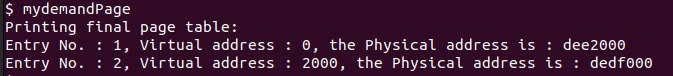
\includegraphics[width=1\textwidth]{1}
	\end{figure}
Number of pages = $2$.
\item For global array of size $3000$
	\begin{figure}[H]
	\centering
	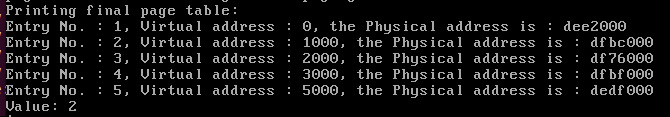
\includegraphics[width=1\textwidth]{2}
\end{figure}
Number of pages = $5$.
\item For global array of size $5000$
\begin{figure}[H]
	\centering
	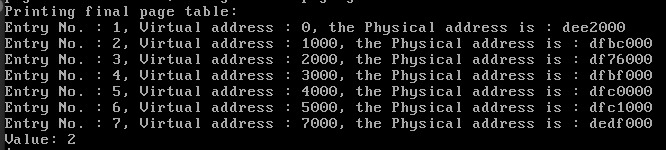
\includegraphics[width=1\textwidth]{3}
\end{figure}
Number of pages = $7$.
\item For global array of size $10000$
\begin{figure}[H]
	\centering
	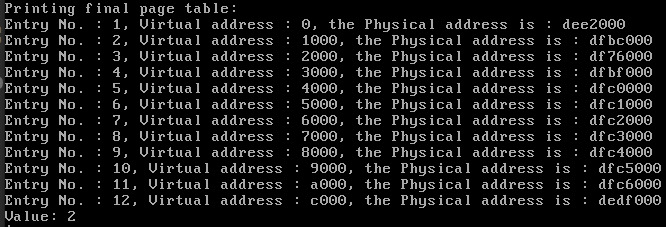
\includegraphics[width=1\textwidth]{4}
\end{figure}
Number of pages = $12$.
\end{itemize}
So, from the above outputs it is clear that as the size of global array increases, size of page table increases.
\end{document}
